%!TEX root = main.tex
\chapter{Results}
\label{chap:results}
In this chapter we will show and discuss the results of the work we have done in this thesis.

We will start by looking at the train and test sets of the four dataset (see \autoref{tab:model_delimitation} and below) and describe what we did about class imbalance. Then we describe and interpret our results and we end the chapter with a brief summary of our findings. 

From \autoref{chap:methods} we have found the following datasets and model pairs based on the available data (see also \autoref{tab:model_overview} and \autoref{tab:model_delimitation}):
\begin{enumerate}
\item Test data
\begin{enumerate}
\item without user-filtering \\\textbf{Model pair: TP-1}
\item with user-filtering using cross-occupancy of 40\% \\\textbf{Model pair: TP-2}
\end{enumerate}
\item Production data
\begin{enumerate}
\item without user-filtering \\\textbf{Model pair: PP-1}
\item with user-filtering using cross-occupancy of 10\% \\\textbf{Model pair: PP-1}
\end{enumerate}
\end{enumerate}


For our test data without user-filtering we found a training set with 1798 negative samples (did not meet) and 9203 positive samples (did meet). In our test set we found a more moderate 5513 negative samples (did not meet) and 1674 positive samples (did meet).

Using test data with user-filtering in just September we found a training set with 118 that did not meet and 95 that did meet. The test set consisted of 151 that did not meet and 98 that did meet. 

Using production data without user-filtering we found 5585 that did not meet and 10907 that did meet for our training set, for our test set we found 9148 that did not meet and 10028 that did meet.

Using production data with user-filtering we found 403 that did not meet and 4533 that did meet for our train set and 402 that did not meet and 4630 that did meet for our test set.

The datasets composed from the test data have more negative samples than positive samples. In TP-1 the difference is more pronounced than in TP-2, except of the training set. In the production data, we have the opposite. Here we have more positive samples than negative. \\
This shows we have a class impalance problem since the dataset are imbalanced. Due to this, the Logistic Regression classifier we trained initially predicted the largest prevalent class, in our training dataset. The next section explains this problem and how we dealt with it. 


\section{Class Imbalance Problem}
\label{sec:class_imbalance_problem}
The Class Imbalance Problem is when the total number of samples for one class greatly exceeds the number of samples for a different class. A number of techniques can be used to handle the class imbalance problem, we will use two techniques called oversampling and undersampling\cite{tan2006introduction}. In oversampling you sample the minor sample with replacement until there is an equal number of positive and negative samples. In undersampling you randomly sample from the major class $N$ times where $N$ is the number of minor classes.

\section{Performance metrics}
\label{sec:performance_metrics}
We utilize the precision and recall metrics for evaluating the performance of our models as well as AUC of the ROC Curve.

\subsection{Receiver Operating Characteristic (ROC)}
The Receiver Operating Characteristic or ROC in short, illustrates the performance of a binary classifier in terms of the true positive rate (TPR, also called recall) plotted against the false positive rate (FPR) at different discrimination thresholds. As points on the ROC-curve represents different thresholds with an associated (TPR,FPR) pair it allows us to see different trade offs between TPR and FPR. The ROC curve is useful for comparing the relative performance of different classifiers\cite{tan2006introduction} The area under the curve (AUC) represents the probability that a classifier will rank a random positive sample higher than a negative sample, assuming positive ranks higher. An AUC of 0.5 would mean the model would just randomly guess the class of each sample. We will use the ROC AUC as a metric for comparing our different models.

\subsection{Precision and Recall}
Precision or the positive predictive value (PPV) is a metric that measures the number of a given class that are correctly identified in proportion to the number of classes that are predicted to be that class.
%\subsection{Recall}
\textcolor{blue}{Recall}
Recall or the true positive rate (TPR) is a metric that measures the number of a given class that are correctly identified as that class.

In Table \ref{table:models_performance_report} we can see the performance metrics of the different classifiers for the positive (did meet) and negative class (did not meet).

\begin{table}[H]
\centering
\begin{tabular}{|c|c|c|c|c|c|c|c|c|c|c|}
\hline
\textbf{Model} & \textbf{PPV +} & \textbf{TPR +} & \textbf{PPV -} & \textbf{TPR -}   \\
\specialrule{.20em}{.0em}{.0em}
LR in TP-1    & 0.25 & 0.67 & 0.86 & 0.51\\
\hline
RF in TP-1    & 0.28 & 0.53 & 0.85 & 0.67\\
\specialrule{.15em}{.0em}{.0em} 
LR in TP-2    & 0.53 & 0.68 & 0.70 & 0.56\\
\hline
RF in TP-2    & 0.52 & 0.59 & 0.68 & 0.60\\
\specialrule{.15em}{.0em}{.0em}
LR in PP-1    & 0.66 & 0.74 & 0.54 & 0.44\\
\hline
RF in PP-1    & 0.66 & 0.55 & 0.51 & 0.58\\
\specialrule{.15em}{.0em}{.0em}
LR in PP-2    & 0.94 & 0.81 & 0.17 & 0.40\\
\hline
RF in PP-2    & 0.94 & 0.92 & 0.26 & 0.34\\
\hline
\end{tabular}
\caption{Models performance metrics}
\label{table:models_performance_report}
\end{table}

We can further look at the number of classes correctly and incorrectly predicted using a Confusion Matrix. Figure \ref{fig:conf_matrix_log_reg} and \ref{fig:conf_matrix_random_forest} shows the confusion matrices for our two models.

\begin{figure}[H]
    \hspace*{-1.0cm}
    \centering
    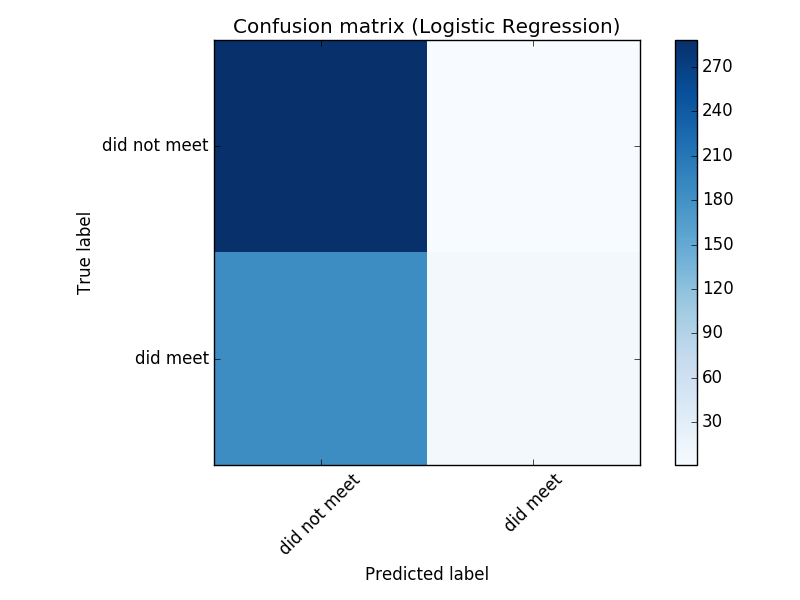
\includegraphics[scale=0.50]{confusion_matrix_log_reg}
    \caption{Confusion matrix for Logistic Regression (num\_coocs feature)}
    \label{fig:conf_matrix_log_reg}
\end{figure}
\begin{figure}[H]
    \hspace*{-1.0cm}
    \centering
    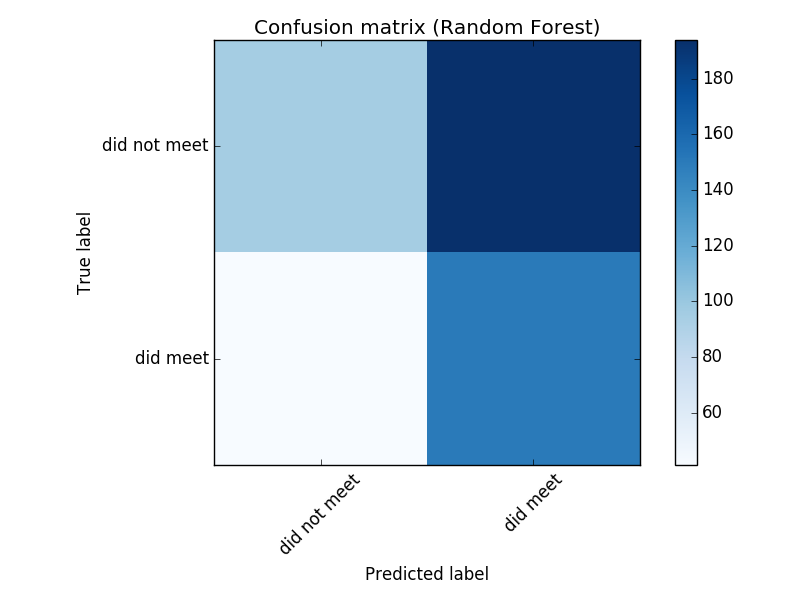
\includegraphics[scale=0.50]{confusion_matrix_random_forest}
    \caption{Confusion matrix for Random Forest (all features, 200 trees)}
    \label{fig:conf_matrix_random_forest}
\end{figure}

Looking at Figure \ref{fig:conf_matrix_log_reg} we see our baseline classifier has a very high BLABLA

\subsection{Feature importance}
We can plot the feature importances of the random forest classifier
\begin{figure}[H]
    \hspace*{-1.0cm}
    \centering
    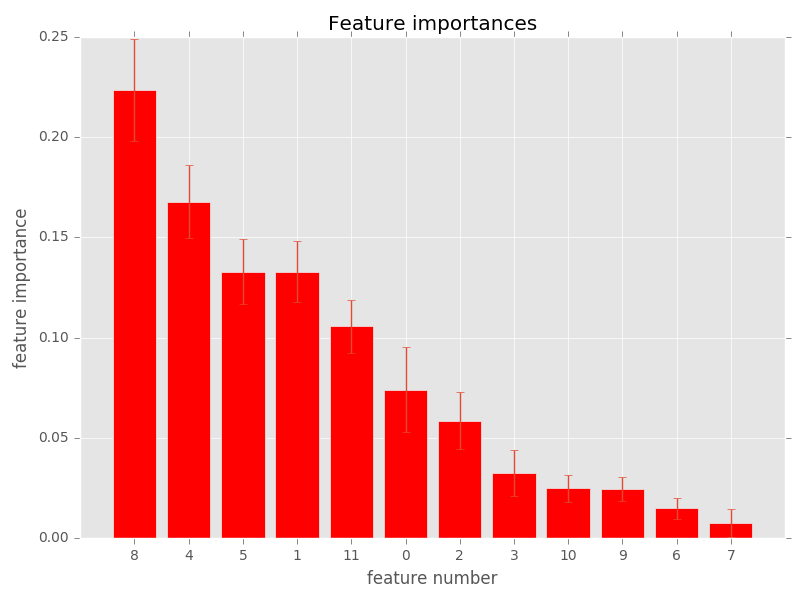
\includegraphics[scale=0.40]{feature_importances}
    \caption{Feature importances of random forest}
    \label{fig:feature_importances}
\end{figure}

In Figure \ref{fig:rocs} we have plotted the ROC curve and ROC AUC for the different model pairs, we have also plotted the curve of a randomly guessing classifier for comparison. Figure \ref{fig:rocs_undersampling} shows the same models performance, where the datasets most prevalent class have been undersampled.

\begin{figure}[H]
    \hspace*{-1.0cm}
    \centering
    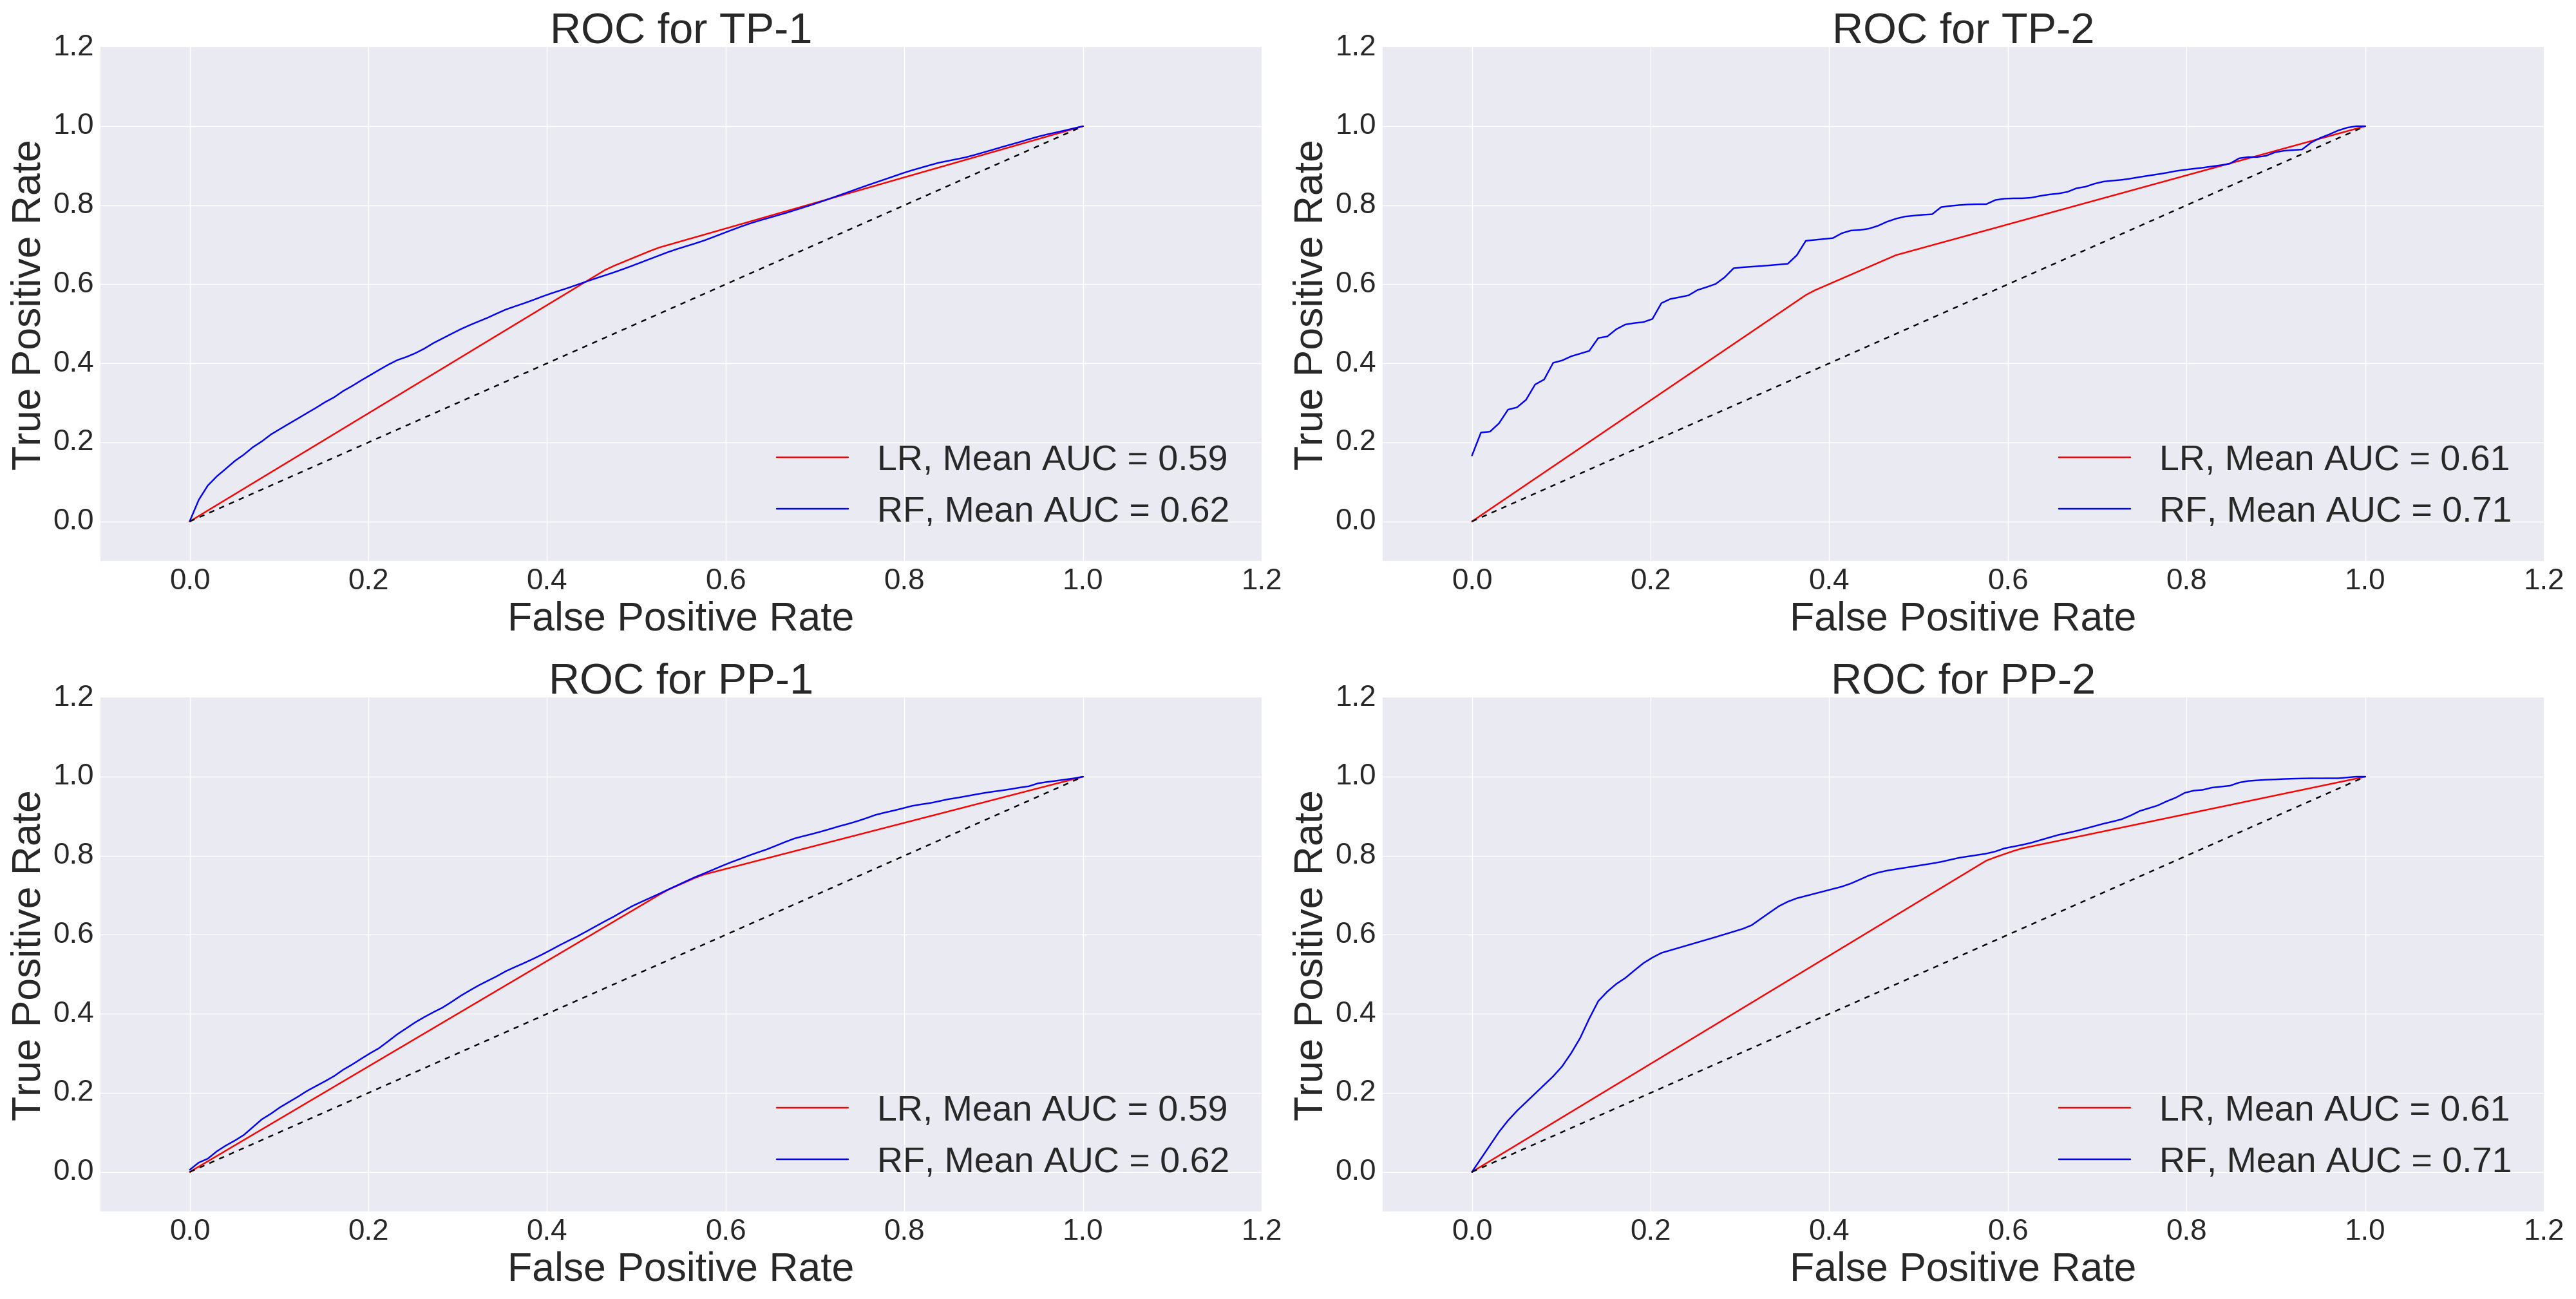
\includegraphics[scale=0.15]{ROCS}
    \caption{mean ROC AUC of Logistic Regression (LR) and Random Forest (RF) in the four model-pairs (TP-1, TP-2, PP-1, PP-2) using randomized search for hyper-parameter optimization (internal loop with 3-fold cross-validation) and 2-fold cross-validation. }
    \label{fig:rocs}
\end{figure}
\begin{figure}[H]
    \hspace*{-1.0cm}
    \centering
    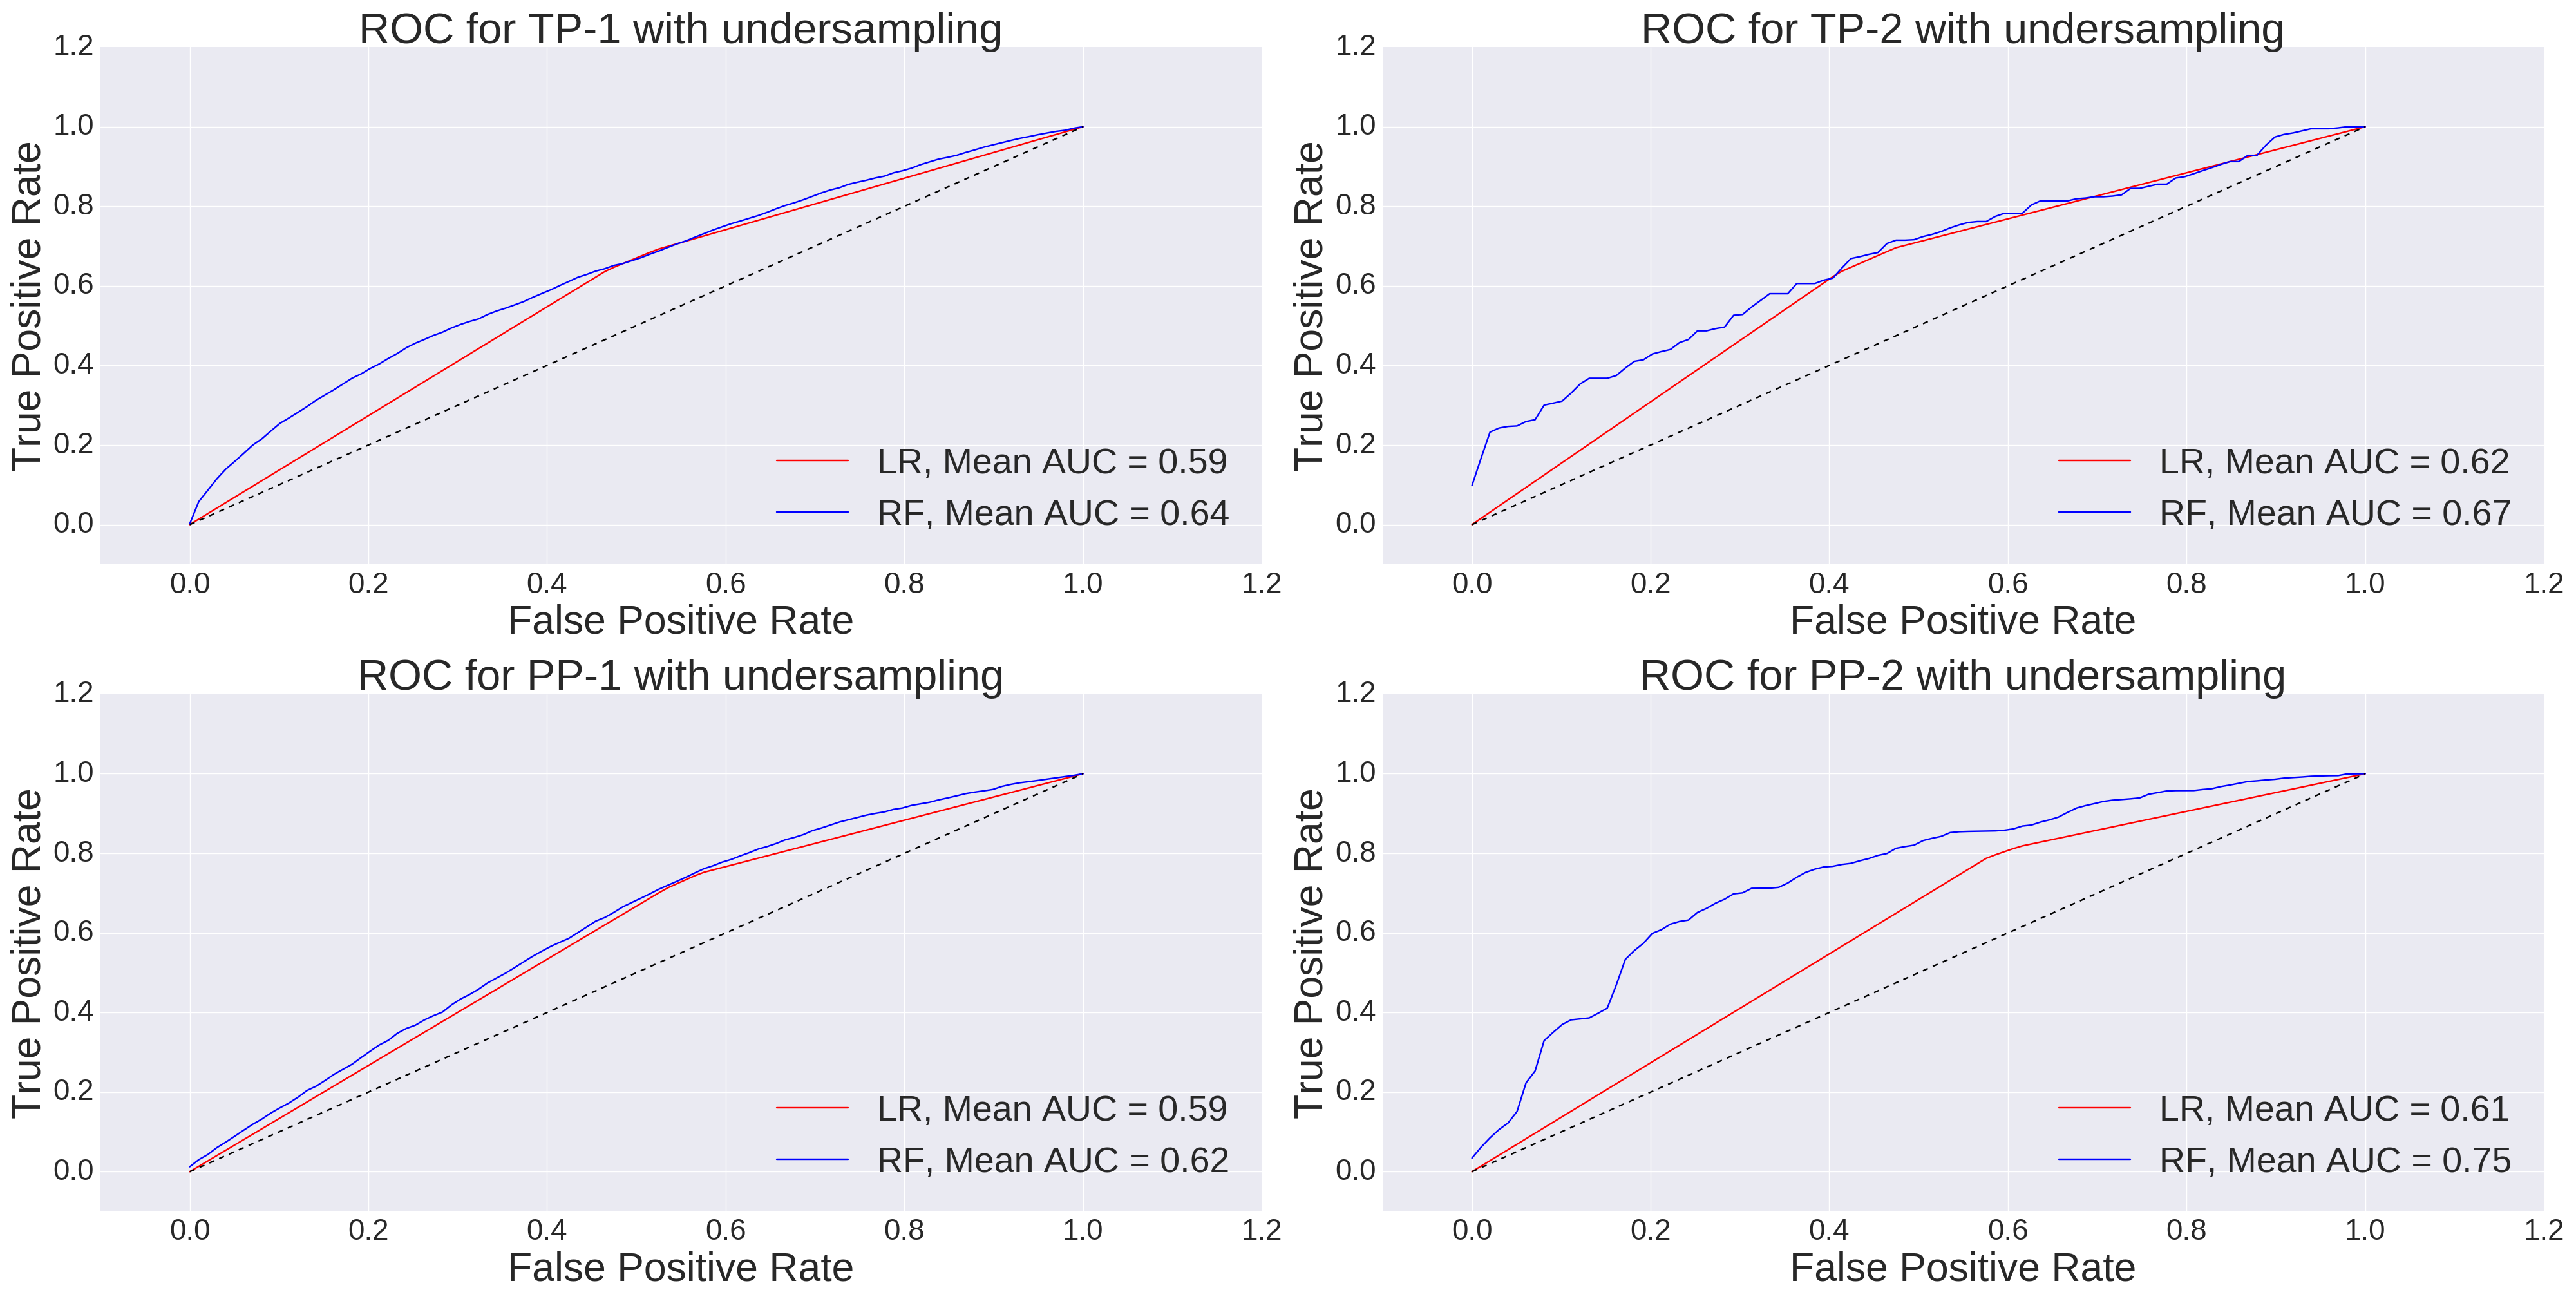
\includegraphics[scale=0.15]{ROCS_undersampling}
    \caption{mean ROC AUC of Logistic Regression (LR) and Random Forest (RF) in the four model-pairs (TP-1, TP-2, PP-1, PP-2) using randomized search for hyper-parameter optimization (internal loop with 3-fold cross-validation) and 2-fold cross-validation, and with undersampling of the most prevalent class}
    \label{fig:rocs_undersampling}
\end{figure}
\section{Summary}